\section{投机BFT:Ouroboros-BFT与Zyzzyva}
对BFT的高通信复杂度优化的思考引出了一系列所谓投机BFT算法,即,在更强的假设前提下(网络环境更好或拜占庭节点更少)能有更好的性能(performance)。
\subsection{Zyzzyva}
Zyzzyva\cite{kotla2007zyzzyva}由Lorenzo等人在2007年提出,发表在SOSP上并被评为Best Paper。这个命名据说是选取的字典表里的最后一个单词,意味着Zyzzyva是这一系列算法的终结(然而之后还是出现了更好的算法)。

Zyzzyva的协议分为检查点(checkpoint)协议,视图转换(view change)和一致性(agreement)协议。这里我们介绍后两部分。

Zyzzyva其大致结构和定义和PBFT类似,($f$个拜占庭节点,一共$3f+1$个节点,异步网络模型)实现的目标是能有更快的消息复杂度,其核心思想在于在请求的确定被完全确定之前就开始执行。
\subsubsection{流程}
\begin{itemize}
	\item 1. 客户端发送请求给主节点
	\item 2. 主节点接受到请求,给其设置编号,并将请求广播到所有副本节点。
	\item 3. 副本节点接收到有序(ordered)请求,并投机的执行它们,并且给客户点发送回复。
	\item 4. 客户端开始接受副本节点发出的回复,根据\emph{一定时间内}收到的回复数量可以分为下面三种情形:
	   \begin{itemize}
	   	    \item 4a. 若客户端收到$3f+1$个回复(和他的请求匹配的),则认为请求被成功执行,完成请求(complete the request)
	   	    \item 4b. 若客户端收到的回复个数在$2f+1$和$3f$之间,则其生成一个commit信息(包含发送这$2f+1$个回复的节点的ID,签名,请求内容等),并广播给所有的副本节点
	   	        \begin{itemize}
	   	    	\item 4b.1 当副本节点接收到一个合法的commit信息时,生成一个local-commit信息并发送给客户端(若收到的commit信息包含的记录和本地记录不一致,则发起view change(更换主节点))
	   	    	\item 4b.2 当客户端收到$2f+1$个合法的local-commit信息时,完成请求。系统能保证即使存在view change,所有诚实的副本节点都会执行请求。(若客户端在限定时间内没有收到$2f+1$个local-commit信息则跳入4c步骤)
	   	    	\end{itemize}
	   	    \item 4c. 若客户端收到的回复个数少于$2f+1$个,则客户端将请求重新发送给所有副本节点并抄送给主节点(以获得序号)。
	   	     \begin{itemize}
	   	    \item 4c.1 当副本节点收到客户端的请求信息时,若该请求拥有最高的时间戳(timestamp),	则副本节点再发送一个confirm-req信息给主节点$p$并开始计时。若在限定时间内收到主节点发送的有序请求(order-req),则如前所述正常执行该请求。若在限定时间内没有收到,则发起view change,同时将confirm-req广播到所有副本节点。\footnote{注意到这里出现了$n^2$级别消息传输复杂度。}副本节点收到confirm-req时向发送方发送从主节点发来的有序请求。
	   	    \item 4c.2 当主节点收到confirm-req信息时,主节点如第二步所述发送有序请求。
	   	    \end{itemize}
	   	    \item 4d 当客户端发现请求不一致时,发送proof-of-mistake(POM)给所有副本节点并开始view change。(文章提到发起view change并不会影响请求被执行)
	   	\end{itemize}	
\end{itemize}

Zyzzyva的视图转换协议运作当且仅当下面两种情况发生
\begin{itemize}
	\item 当主节点查出有拜占庭行为
	\item 当$f+1$个节点发起view change(文中的方式为发送i-hate-the-primary信息)
\end{itemize}
\reffig{fig:zyzzyva1}演示了Zyzzyva的共识流程。

\begin{figure}
	\centering
	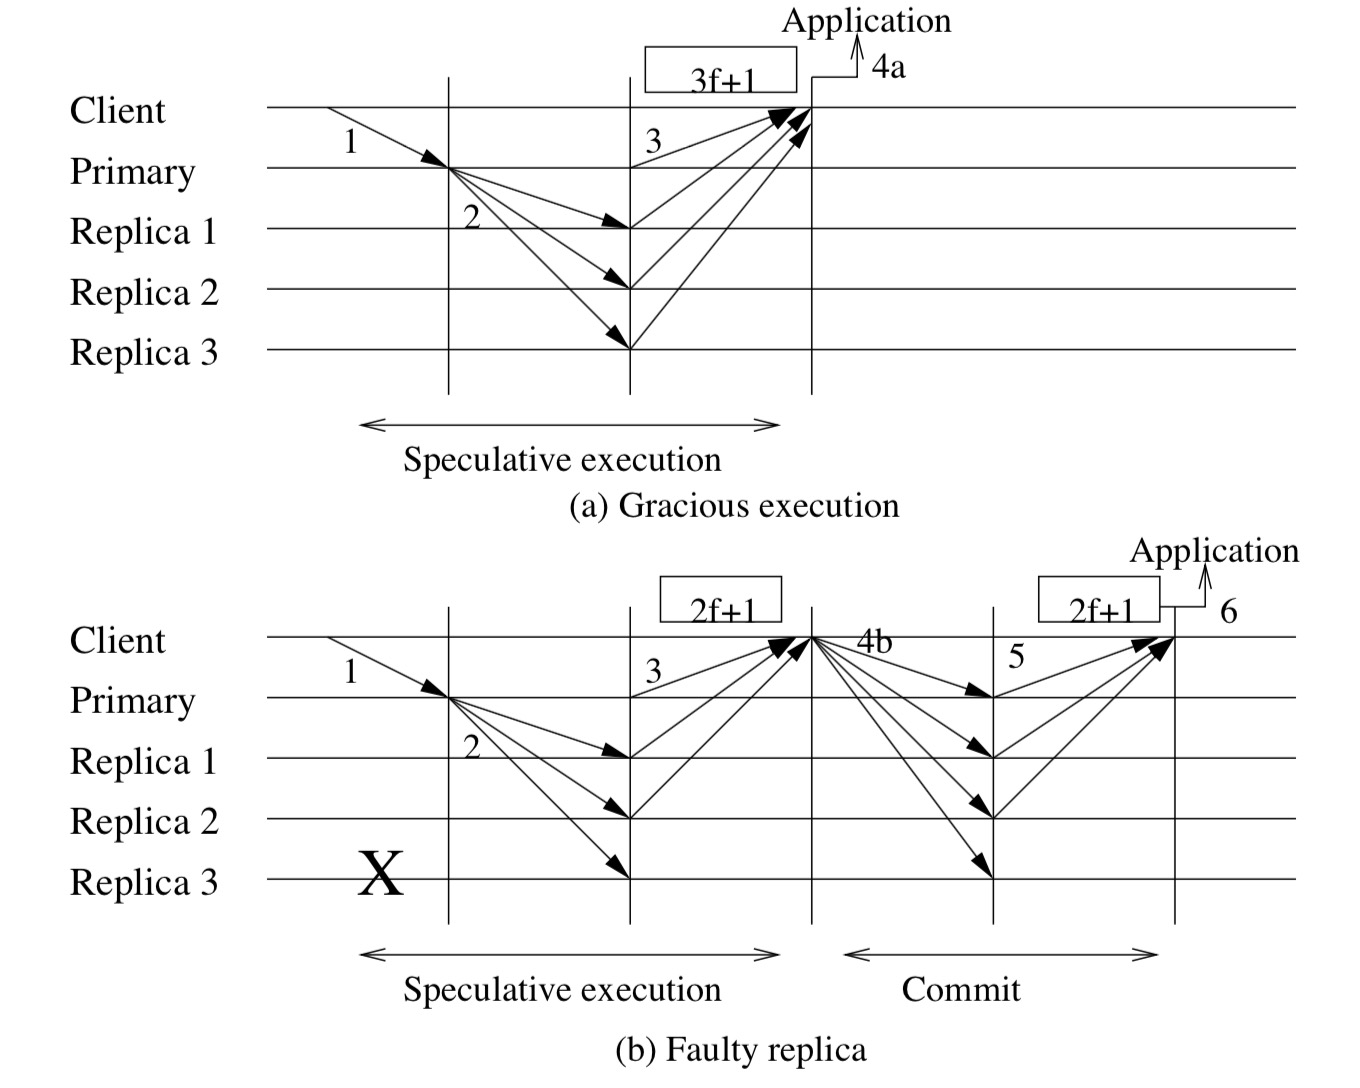
\includegraphics[width=0.8\textwidth]{../common/zyzzyva_1.png}
	\caption{Zyzzyva共识算法流程} 
	\label{fig:zyzzyva1}
\end{figure}

文章之后给出了安全性及一致性的证明,以及用实验对比PBFT的性能。这里不详细介绍。

\subsubsection{总结}
Zyzzyva和PBFT相比,运气好的时候执行的更快,但是当主节点更换频繁时效果可能更差。

值得一提的是,Zyzzyva团队之后又提出了致力于在更多的拜占庭故障发生时也能保持高性能的算法,发表在2009年NSDI上\cite{clement2009making},称作Aardvark,据说是字典表的第一个单词(表达他们已经经历了一个轮回)。

\subsection{Ouroboros-BFT}
Ouroboros-BFT由Ouroboros(Cardano项目,代币名称: ADA)团队于2018年9月提出\cite{kiayias2018ouroboros}。Ouroboros-BFT和他们本身的Ouroboros共识(会在下个部分介绍)联系不大,仅仅是提出一种投机BFT协议。

文章解决的是区块链的共识问题。文章的主要贡献是提出一种交易确认时间极快(通常为$O(t)$,$t$为拜占庭节点数目),传播复杂度较小(最优情况为$O(n)$,最坏情况为$O(nt)$),容错为$t\leq n/3$的共识协议。

\textbf{假设}

Ouroboros-BFT与传统BFT算法最大的不同是他对网络环境做了很强的假设,主要在以下两个方面:
\begin{itemize}
	\item 文章所有的结论都是在同步网络模型下进行分析。文章假设任何异步网络环境都是暂时的,一旦网络环境回归同步,则共识协议会收敛回安全状态。
	\item 文章假设存在一个全局同步的时钟,并在文章的最后给出了如何模拟这个时钟的方法。
\end{itemize}

\textbf{算法}

Ouroboros-BFT将时间看做若干个时间段$sl_1,sl_2,\cdots$,并假设该时间段发出的消息能在下个时间段被所有的服务器接受。同时,每个服务器维护一个区块链$B_0,B_1,...$,其中$B_i$包含的信息为前一个区块哈希值,当前的时间段,打包的所有交易,对时间段的签名,

具体算法如下:
\begin{enumerate}
	\item 当服务器收到一笔合法的交易$tx$时,将其放到交易池里面,其在交易池中“存活”$u$个时间段。服务器可以选择性的给客户端回复一个收据用以确认交易。
	\item 当服务器意识到一个更长的区块链的存在时,若验证了其合法性(主要验证区块提出者编号等于时间戳$mod~n$),用之替换其本地的区块链。
	\item 当服务器发现轮到自己出块时(同上,编号同余于时间戳),打包所有交池中交易,并且按照格式进行签名同时广播区块。
	\item 当服务器收到询问请求时,回复已被最终确认(finalize)的区块
	\item 当客户端收到$r$个针对某交易的收据时,则该交易被最终确认。
\end{enumerate}
文章接下来分析协议的活性,一致性保证等等。结论主要在以下两个方面:
\begin{enumerate}
	\item Ouroboros-BFT能保证一致性和参数为$5t+2$的活性,即任何交易都会在$5t+2$个时间段内被打包
	\item Ouroboros-BFT能保证参数为$5t+2+n-r$的确认时间,即任何交易都会在$5t+2+n-r$个时间段内被最终确认。
\end{enumerate}
文章之后还研究了一种covert设定\cite{aumann2007security},具体读者可参阅原文这里不做详细介绍。

\textbf{总结}
Ouroboros-BFT因为强假设太多,实际可参考价值并不大,更多的是提供了一种基于全局时钟的处理方案。根据分布式经典论文\cite{lamport1978time}中的介绍,实际中能够确定的只是行为间的偏序关系(Partial order),往往会存在多个符合给定偏序关系的全局顺序。通常的假设是每个进程有一个本地的时钟,但可以在信息交换的过程中不断维护和更新本地时钟。故全局时钟的存在是一种理想的环境。当然,全局时钟的设定目前也被一些其他文献所接受,如google的~\cite{burrows2006chubby,corbett2013spanner}。而在区块链中,通常以区块高度或类似的,轮数(round)这种全局变量来实现全局时钟的效用。

文章还提到了SBFT\cite{golan2018sbft} (2018年, cite 9次),另外一种投机BFT算法。


\subsection{总结与思考}
投机BFT属于基于PBFT的扩展,但我们认为实际操作中还是PBFT更具参考价值。但是鉴于大部分公链难以承受PBFT的高复杂度,需要针对具体环境进行优化。投机BFT给出了优化的参考方案。

事实上,本部分提到的所有文献除了Ouroboros-BFT,都不是关于区块链的。他们解决的是更为本质的状态机复制问题,而大量区块链项目仍然需要对网络环境作一定量的假设,这在下部分介绍中可以看到。作为区块链共识协议的设计者,需要了解状态机复制的工作原理和基本方法,将其作为一种最高要求的实现,但同时也不需要拘泥于此,适当的对网络环境做出假设,以牺牲一部分理论高度来换取应用于实际的性能是更为可行的方案。